\section{Model Exercise 3-2: Constant normal stiffness (CNS) direct shear test}
\label{sec:mex08}
%------------------------------------------------------------------------------
\Authors{Daniel P\"otschke, Thomas Fr\"uhwirt et al.}
%------------------------------------------------------------------------------
\subsection{Experimental set-up}
%------------------------------------------------------------------------------
\begin{figure}[!ht]
\begin{center}
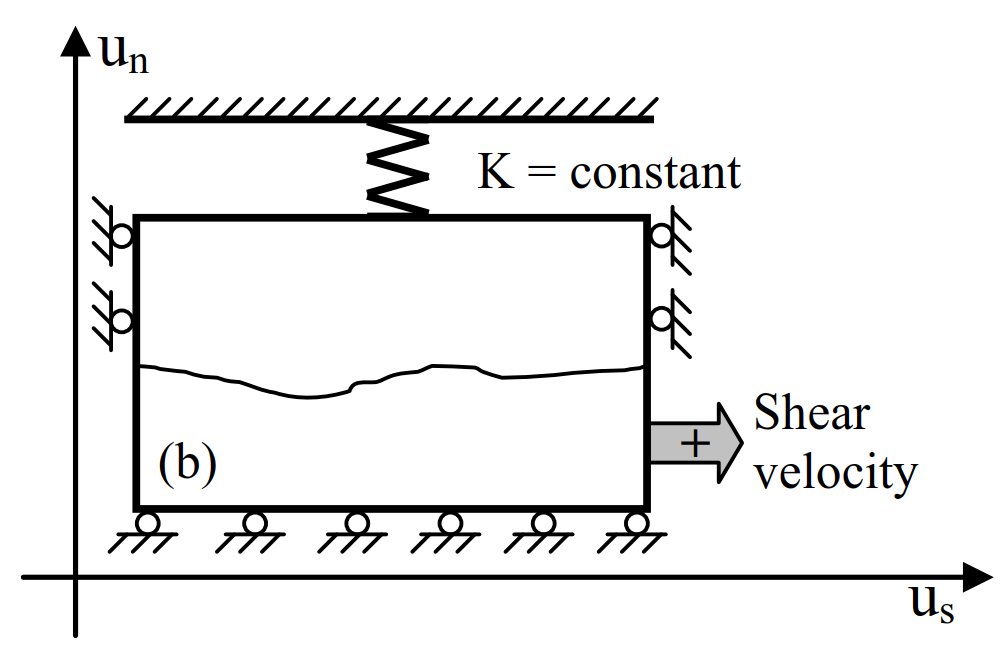
\includegraphics[width=0.5\textwidth]{./figures/MEX8_CNS_Nguyen_Thesis.PNG}
\end{center}
\caption{Constant normal stiffness (CNS) direct shear test. (From: \cite{Nguyen2014})}
\label{fig:MEX8_CNS}
\end{figure}

Constant normal stiffness (CNS) direct shear tests follow the same basic principles like CNL tests (\ref{sec:mex07}). Additionally to the initial normal load an extra load is added when the rock joint opens. This situation is comparable to a rock joint in the underground where surrounding rock masses have to be deformed to open a joint. This deformation causes the extra loads. In \ref{fig:MEX8_CNS} the stiffness term is represented as a spring with a constant stiffness. The difficulty is how to estimate this stiffness. If the focused joint is surrounded by intact rock material it will be higher than for a jointed, weathered surrounding. A CNL test is a CNS test for which the stiffness is zero. This situation marks the lower boundary of the stiffness and is a valid boundary condition for rock joints close to the surface. The upper boundary of the stiffness is the stiffness of the intact rock. The real situation will be somewhere in between this extreme cases.\\
The expected result is that for higher stiffness values the shear forces increase due to the increasing normal load when the joints starts to open.\\
The input data for this model exercise are similar to the data for the CNL test. Basic rock parameters for the basalt sample [table], the surface scan data [also for CNL: How to provide this - external download link?] and the boundary conditions of the lab investigations. The aim is to use this input to make good back calculations of the lab data. A good modelling approach for CNS tests can also used for CNL tests by simply setting the stiffness as zero.


%------------------------------------------------------------------------------
\subsection{Model approach}
%------------------------------------------------------------------------------
Additionally to the model approach for CNL tests an estimation of the dilation is needed. The normal stress has to be updated once the dilation is known.\\

%------------------------------------------------------------------------------
\subsection{Results and discussion}
%------------------------------------------------------------------------------

\todo[inline]{[TUBAF] Please complete section}